\renewcommand{\theequation}{\theenumi}
\begin{enumerate}
\numberwithin{equation}{enumi}

\item \begin{flushleft}
Let $\vec{E}$ be a point which divides line segment $AB$
in the ratio $k : 1$ :
\end{flushleft}

\item \begin{align}
\vec{E} &= \frac{k\vec{A}+\vec{B}}{k+1}
\end{align}

\item \begin{flushleft}
$\vec{C}$ divides the line in the ratio $\frac{1}{2} : 1 $ and $\vec{D}$ divides the line in the raio $\frac{2}{1} : 1 $
\end{flushleft}

\item \begin{align}
\vec{C} &= \frac{0.5\vec{A}+\vec{B}}{0.5+1} \\
\vec{D} &= \frac{2\vec{A}+\vec{B}}{2+1}\\
\therefore \vec{C} &= \myvec{0\\-2.33}\\
\therefore \vec{D} &= \myvec{2\\-1.66}
\end{align}

\item \begin{figure}[!ht]
\centering
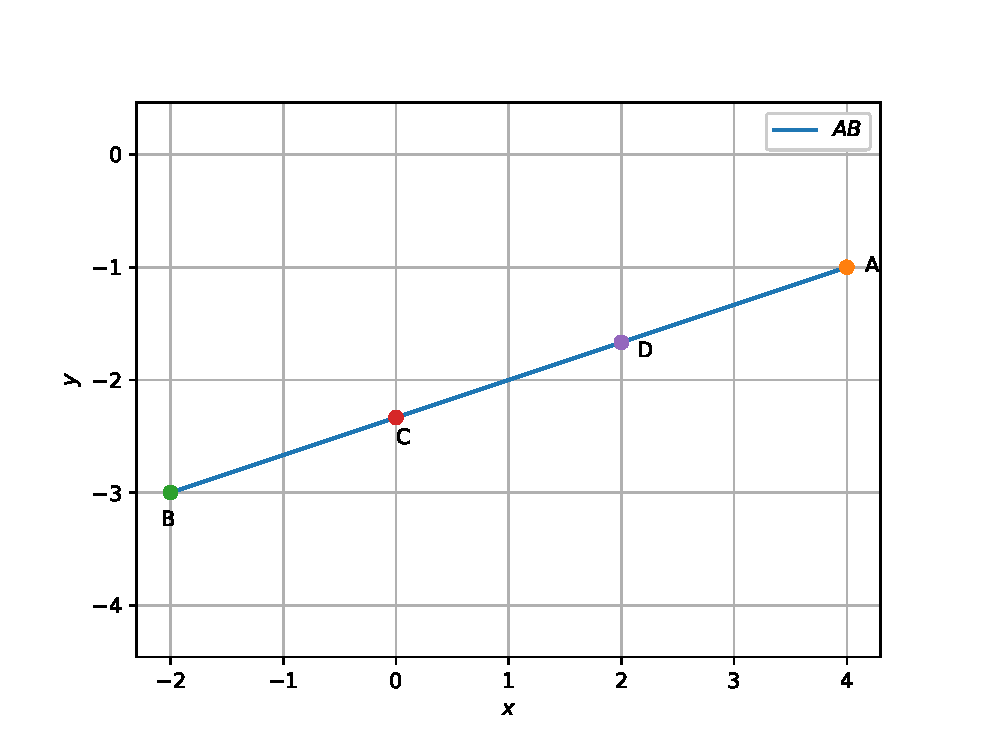
\includegraphics[width=\columnwidth]{./figs/line_ex/pts_on_a_line/trisection.eps}
\caption{Line $AB$ trisected - generated using python}
\label{fig:trisection_pts_on_a_line}
\end{figure} 

The following Python code generates Fig. \ref{fig:trisection_pts_on_a_line}

\begin{lstlisting}
codes/line_ex/pts_on_a_line/trisection.py
\end{lstlisting}
\end{enumerate}